\documentclass[12pt]{article}

\usepackage[a4paper,left=2.5cm,right=2.5cm,top=2.5cm,bottom=2.5cm]{geometry}
% \usepackage[bahasa]{babel}
\usepackage[style=apa]{biblatex}
\addbibresource{main.bib}

\usepackage{titlesec}

\titleformat{\section}
  {\normalfont\fontsize{13}{15}\bfseries}{\thesection}{1em}{}

\renewcommand\thesection{\Alph{section}.}
% \renewcommand\thesubsection{\thesection.\Alph{subsection}}

\usepackage{setspace} \onehalfspacing
\usepackage{lipsum}
\usepackage{graphicx}
\usepackage{hyperref}
% \usepackage{biblatex}
% \addbibresource{main.bib}
% \usepackage{apacite}
\usepackage{longtable}
% \usepackage[backend=biber,style=apa,citestyle=apa,sorting=ynt]{biblatex}
\usepackage{usebib} 
\bibinput{main}
\usepackage{indentfirst}
\graphicspath{ {./images/} }
\title{Tugas Sistem Jaringan Bisnis Internasional}


\begin{document}
\thispagestyle{empty}
\begin{center}
    Tugas\\
    \textbf{Sistem Jaringan Bisnis Internasional }\\
    Singaporean Dollar (SGD) terhadap Indonesian Rupiah (IDR)\\
    \vspace*{11\baselineskip}
    
\includegraphics[width=0.4\textwidth,height=0.4\textwidth]{glogo}  \\
    \vspace*{11\baselineskip}
    disusun oleh:\\
    \textbf{Ilman Samhabib (91122010)}\\
    \textbf{Universitas Gunadarma}\\
    \textbf{2023}\\
\end{center}
\newpage

\section{Pendahuluan}


Tulisan ini mencoba menggali dinamika rumit yang memengaruhi apresiasi dan depresiasi Dolar Singapura (SGD) terhadap Rupiah Indonesia (IDR) selama periode 2021 hingga 2022. Uraian ini meliputi berbagai kekuatan yang membentuk pergerakan nilai tukar kedua mata uang ini, dengan memeriksa indikator ekonomi, perbedaan suku bunga, neraca perdagangan, stabilitas politik, kondisi ekonomi global, spekulasi pasar, dan kebijakan moneter.

\section{Analisis Nilai Tukar}
\begin{center}
    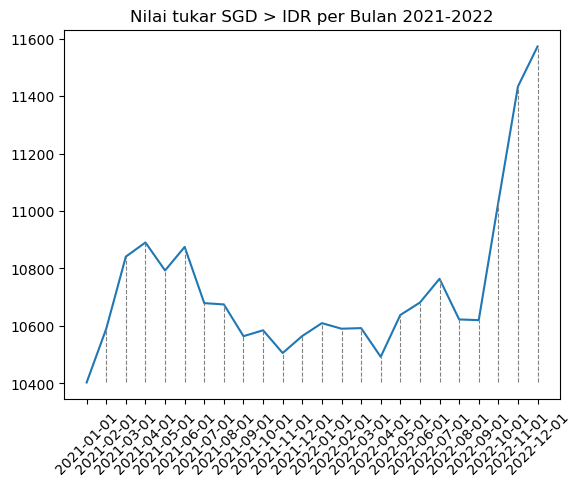
\includegraphics[width=0.7\textwidth,height=10cm]{monthly-graph-2}
\end{center}

\subsection*{Dolar Singapura Menguat Sedikit (Januari-April 2021)}

\begin{enumerate}
    \item \textbf{Penguatan Dolar Singapura (SGD):}
    \begin{itemize}
        \item Nilai tukar Dolar Singapura tercatat menguat sepanjang kuartal I-2021, walaupun tidak signifikan. Perekonomian Singapura yang diprediksi keluar dari resesi memberikan kekuatan pada mata uangnya.
        \item Menurut data Refinitiv, SGD menguat sebesar 1,6\% selama tiga bulan pertama tahun ini. Pada 31 Maret 2021, SGD mencapai Rp 10.794,74/SG\%, mencapai level tertinggi sejak 23 Oktober 2020.
        \item Pada 1 April 2021, SGD naik tipis 0,1\% ke Rp 10.804,19/SG\%.
    \end{itemize}

    \item \textbf{Ekspor dan Pertumbuhan Ekonomi Singapura:}
    \begin{itemize}
        \item Pada pertengahan Maret, data dari Pemerintah Singapura menunjukkan ekspor non-minyak naik 8,2\% secara month-to-month (MtM) dan 4,2\% secara year-on-year (YoY).
        \item Singapura, yang bergantung pada ekspor, memiliki rasio ekspor terhadap Produk Domestik Bruto (PDB) tertinggi di dunia.
        \item Proyeksi pertumbuhan PDB Singapura oleh Bank ING di kuartal I-2021 direvisi menjadi 0,2\%, menandakan keluar dari resesi.
    \end{itemize}

    \item \textbf{Inflasi dan Proyeksi Kedepan:}
    \begin{itemize}
        \item Inflasi di bulan Februari tumbuh sebesar 0,7\% year-on-year (YoY), melebihi konsensus pasar sebesar 0,6\%.
        \item Proyeksi PDB Singapura sepanjang tahun 2021 oleh ING adalah tumbuh sebesar 5,2\%.
    \end{itemize}

    \item \textbf{Kontrast dengan Indonesia:}
    \begin{itemize}
        \item Sementara Singapura mengalami pertumbuhan ekonomi, Indonesia masih belum keluar dari resesi di kuartal I-2021, dengan proyeksi pertumbuhan negatif oleh Kementerian Keuangan.
        \item Upaya Indonesia untuk mengatasi resesi masih menjadi fokus, sementara Dolar Singapura mengalami apresiasi yang lebih moderat.
    \end{itemize}
\end{enumerate} \autocite{Putu_Agus_Pransuamitra_2021_APRIL_cnbcindonesia}

\subsection*{Stagnan pada Pertengahan 2021 sampai Pertengahan 2022}

Dolar Singapura mengalami fluktuasi pekan ini, dengan rentang pergerakan yang cukup luas, tetapi pada akhirnya hanya mencatat penguatan atau pelemahan tipis. Meskipun volatilitas yang mencolok, mata uang tersebut mengakhiri pekan dengan penguatan atau pelemahan yang minim.

Di awal pekan, dolar Singapura diperdagangkan dalam kisaran Rp 10.419 - 10.489/SG\$, tetapi akhirnya berada di Rp 10.465/SG\$, menunjukkan kenaikan 0,07\%. Volatilitas ini terkait dengan kebijakan pengetatan moneter yang diterapkan oleh Otoritas Moneter Singapura (MAS) bulan lalu, yang mengubah titik tengah dan menaikkan slope. Pelaku pasar menantikan respons kebijakan Bank Indonesia (BI) terhadap inflasi yang terus meningkat di Indonesia.\autocite{Putu_Agus_Pransuamitra_2021_APRIL_cnbcindonesia}

Dalam laporan terpisah, dolar Singapura mengalami kesulitan untuk menguat di atas Rp 10.600/SG\$ sejak 3 Agustus. Meskipun pembatasan sosial dilonggarkan, dolar Singapura tidak mampu menembus level tersebut. Langkah-langkah pelonggaran melibatkan peningkatan vaksinasi, namun nilai tukar dolar Singapura tetap tertekan. Dari perspektif teknis, dolar Singapura menunjukkan tanda-tanda tekanan, termasuk potensi munculnya death cross. Artikel ini mencatat stagnasi dan pelemahan dolar Singapura dalam konteks teknis dan fundamentalnya.\autocite{Putu_Agus_Pransuamitra_2022_AUG_cnbcindonesia}



\subsection*{Apresiasi Dolar Singapura (SGD) menjelang akhir 2022}

\begin{enumerate}
    \item \textbf{SGD Mengalami Kenaikan:}
    \begin{itemize}
        \item SGD menunjukkan tren kenaikan yang mengesankan terhadap Rupiah Indonesia (IDR) pada Oktober, mencapai di atas Rp 11.000/SG\%.
        \item Data Refinitiv menunjukkan apresiasi bulanan sebesar 3,8\%, mencatat peningkatan terbesar sejak Juli 2020.
    \end{itemize}

    \item \textbf{Ketatnya Kebijakan Otoritas Moneter Singapura (MAS):}
    \begin{itemize}
        \item MAS telah mengetatkan kebijakan moneter sebanyak lima kali sejak Oktober 2021, dengan penyesuaian terakhir pada Oktober 2022, mengubah pusat nilai tukar efektif nominal dolar Singapura (S\$NEER).
    \end{itemize}

    \item \textbf{Dampak pada Nilai Tukar:}
    \begin{itemize}
        \item Kebijakan ketat memungkinkan SGD untuk lebih menguat lagi, mencapai rekor tertinggi Rp 11.688/SG\% pada 29 Desember 2022.
    \end{itemize}

    \item \textbf{Dinamika Ekonomi Regional:}
    \begin{itemize}
        \item Meskipun Bank Indonesia menaikkan suku bunga acuannya, Rupiah menghadapi tantangan, dengan arus modal keluar dari pasar obligasi akibat ketidakpastian global, terutama di Amerika Serikat.
    \end{itemize}

    \item \textbf{Pendekatan Agresif MAS:}
    \begin{itemize}
        \item Pendekatan ketat MAS berkontribusi pada ketahanan SGD dan diperkirakan akan terus kuat dalam konteks regional.
    \end{itemize}

    \item \textbf{Carry Trade dan Anomali Tingkat Bunga:}
    \begin{itemize}
        \item Tingkat bunga yang lebih tinggi di Singapura menarik strategi carry trade, dengan harapan bahwa SGD akan unggul secara regional.
        \item Sebuah anomali teramati ketika tingkat bunga deposito USD di Singapura melampaui tingkat bunga di Indonesia, mempengaruhi aliran valuta asing.
    \end{itemize}

    \item \textbf{Tekanan pada Rupiah:}
    \begin{itemize}
        \item Eksportir Indonesia diduga menempatkan pendapatan mereka dalam USD di Singapura, tertarik oleh tingkat bunga deposito yang lebih tinggi, berkontribusi pada depresiasi Rupiah.
    \end{itemize}

    \item \textbf{Anomali Mata Uang dan Dampak Ekonomi:}
    \begin{itemize}
        \item Kondisi tidak biasa, seperti kekuatan SGD dan perbedaan tingkat bunga, menciptakan anomali dalam pasar mata uang, mempengaruhi stabilitas Rupiah meskipun surplus perdagangan Indonesia.
    \end{itemize}

    \item \textbf{Outlook ke Depan:}
    \begin{itemize}
        \item Analis memprediksi bahwa SGD mungkin terus mendominasi secara regional, didukung oleh daya tariknya untuk carry trade, sementara ketidakpastian dalam kebijakan moneter global, terutama di AS, terus memengaruhi dinamika mata uang regional. \autocite{Putu_Agus_Pransuamitra_2022_NOV_cnbcindonesia} \autocite{Putu_Agus_Pransuamitra_2022_DEC_cnbcindonesia}
    \end{itemize}
\end{enumerate}


\section{Penutup}
 Fluktuasi nilai tukar antara Dolar Singapura (SGD) dan Rupiah Indonesia (IDR) menggambarkan dampak kebijakan moneter, dinamika ekspor, dan faktor fundamental ekonomi. Kebijakan pengetatan moneter oleh Otoritas Moneter Singapura (MAS) telah memainkan peran kunci dalam pergerakan SGD, sementara respons Bank Indonesia (BI) terhadap inflasi di Indonesia juga menjadi faktor penentu. Volatilitas ini mencerminkan sensitivitas pasar terhadap kebijakan ekonomi dan kondisi makroekonomi kedua negara. Selain itu, faktor-faktor seperti pertumbuhan ekspor Singapura dan kondisi pasar global juga turut memengaruhi pergerakan nilai tukar kedua mata uang. Dengan demikian, dinamika kompleks ini menciptakan lingkungan di mana SGD dan IDR saling mempengaruhi, mencerminkan keterkaitan erat antara ekonomi kedua negara.

% \bibliographystyle{apacite}
% \bibliography{main}

\printbibliography[title=Daftar Pustaka]

\end{document}